\documentclass[a4paper, 11pt, titlepage]{jsarticle}
\usepackage{graphicx}
\usepackage[dvipdfmx]{color}
\usepackage{amsmath}
\usepackage{listings}
\usepackage{hyperref}

\title{知能情報実験 I\hspace{-1.2pt}I\hspace{-1.2pt}I グループ 1 \\ テーマ:機械学習で株価予測をしてみる}
\author{225752B PARK CHEOLHWAN \\ 225741G 清水 優馬 \\ 225745K 大石根 竜馬 \\ 225754J 當山 一朗}
\date{\today}

\begin{document}
\maketitle
\tableofcontents
\clearpage

\section{はじめに}
\subsection{概要}
\indent 本レポートは、知能情報実験 III の一環として取り組んだ「機械学習で株価予測をしてみる」というテーマに関する実験の詳細をまとめたものである。本実験の目的は、テクニカル分析を用いて株価の変動を予測し、その有効性を検証することにある。実験ではLSTM(Long Short-Term Memory)モデルを選定し、yfinance APIを利用して日経225の株価データを収集し、データセットの構築から始まり、モデルの選定とパラメータ調整、予測結果の評価と考察に至るまでの詳細な手順を報告している。\\
\indent 実験の結果、LSTMモデルは特に安定している株価データに対して高い予測精度を示しているが、急激な価格変動に対する予測精度の低下が観察された。このため、外部要因を考慮したモデルの改良が必要であると結論付けた。また、実験計画と実行のバランスの重要性を再認識し、次回以降のプロジェクトにおいてはリスク管理と柔軟な対応が求められることを学んだ。\\
\indent 最終的に、LSTMモデルによる株価予測の有効性を確認し、パラメータ調整とデータ前処理の重要性を再認識した。経済ニュースや市場イベントなどの外部要因を考慮したモデル改良が今後の課題となる。また、グループワークを通じてコミュニケーションや役割分担の重要性を学び、これらの知見を次回以降のプロジェクトに活かすことを目指している。このレポートは、LSTMモデルを用いた株価予測の実験を通じて得られた知見を基に、さらなる研究と応用に向けた具体的な方向性を示している。

\subsection{テーマ: 株価予測とは}
\indent 本グループでは、中長期で株式投資をする個人投資家の投資に対して、将来の株価を予測することの判断材料の一つとして機械学習を活用できることを対象問題として設定した。 株価予測とは、市場に出回っている株価の推移を予測することであり、テクニカル分析やファン ダメンタルズ分析を使って予測することが一般的である。今回の実験では、数値データとして扱う ことができるデータの多いテクニカル分析を用いて株価予測を実施する。テクニカル分析とは、参考文献 \cite{tech}によると、移動平均線、株価チャートなど、株価データの「型」(=パターン)を基礎に、相場の先行きを予測することである。これらの要因を分析し、株価の変動を予測することで、投資家は株価の変動から状況を判断し、収益の最大化を目指すことができる。

\section{実験方法}
実験方法としては、下記のような手順で進める予定で進むことにした。
\begin{itemize}
  \item 実験目的:実験を進む前に、実験で進むテーマを明確にし、目的を設定し、テーマとしては、株価予測を選定した。
  \item データセット構築:株価データを取得し、テクニカル分析を行うためのデータセットをYfinance APIを用いて構築し、実験の対象としては、参考文献 \cite{nikei}によると、1321.T(NEXT FUNDS 日経225連動型上場投信)は、株式会社日本経済新聞社が発表している株価指数で、東京証券取引所プライム市場に上場する銘柄のうち株式市場を代表する225銘柄を対象に算出されている連動型上場投信である。企業単独の業績ではあまり影響がでず、日本企業全体の株価状況が一目でわかる指標かつ、多くの投資家が参考しているのもあり今回の実験で選定した。
  \item モデル選定:株価予測に有効なモデルを探すために、資料などを参考にした結果、LSTM(Long Short-Term Memory)モデルを選定した。
  \item パラメータ調整:LSTMモデルのパフォーマンスを最適化するために、いくつかのパラメータを調整した。パラメータ調整としては、エポック数、バッチサイズ、LSTMユニット数、Dense層、学習率、データの正規化を調整した。
  \item 結果:実験結果をまとめ、考察を行い、意図していた実験計画との違いを検討し、まとめを行った。
\end{itemize}
\subsection{実験目的}
\indent 本グループでは、株価予測モデルの有効性を検証することを目的としている。具体的には、テクニカル分析\footnote{テクニカル分析とは、価格や取引量などの過去の市場データを分析することで、将来の価格動向を予測する方法である。}を用いた移動平均線\footnote{移動平均線とは,一定期間の株価の平均値を連続的に計算し、その推移をグラフで表示する方法である。}や株価チャート\footnote{株価チャートとは、株価の変動をグラフ形式で視覚的に表現したものである。これにより、トレンドやパターンを簡単に把握することができ、テクニカル分析において重要な役割を果たす。}のパターン認識を通じて、株価の変動をどの程度正確に予測できるかを明らかにする予定である。また、異なる分析手法やパラメータの組み合わせが予測精度に与える影響を確認し、最適な予測モデルを特定することを目指している。

\subsection{データセット構築}
\indent yfinance APIを用いて、1日あたりの株価データをそれぞれ取得する。取得したデータは、Open(始値)、High(高値)、Low(低値)、Close(終値)、Volume(取引量)、Dividends(配当金)、Stock Splits(株式分割)の 7つのカラムからなる(Date は除く)。また、取得したデータを元に、直近3年間の株価データを取得し、テクニカル分析を行うことができるデータセットを構築する。yfinanceAPIのURLは、参考文献 \cite{yfin}である。\\\\\\
\indent また、Listing \ref{data}は1321.Tの直近5日間のデータを示しているものである。
\lstinputlisting[numbers=left, breaklines=true, basicstyle=\ttfamily\footnotesize, frame=single, caption=1321.Tの直近5日間のデータ, label=data]{./example/data_sample.txt}
\subsection{モデル選定}
\indent 本実験では、株価予測において有効であると判断したLSTM(Long Short-Term Memory)モデルを用いる。株価のデータが時系列データであるため、まずRNN(Recurrent Neural Network)とLSTMの二つのモデルを考慮した。それぞれのモデルには特性と利点があり、最適なモデルを選定するために比較検討を行った。\\
\indent RNNは時間的な依存関係を学習するために設計されたモデルであるが、長期的な依存関係を学習する際に「消失勾配問題」という問題が発生する。これは、時間が経つにつれて勾配が消失し、学習が進まなくなる問題である。この問題により、RNNは長期間の依存関係を効果的に学習することが難しくなる。\\
\indent この勾配消失問題に対処するために開発されたのがLSTMである。LSTMはRNNの構造に改良を加え、情報の流れを効果的に制御するためのゲート機構を導入している。具体的には、入力ゲート、忘却ゲート、出力ゲートの3つのゲートを使用し、重要な情報を保持し、不要な情報を忘却することができる。この設計により、LSTMは長期的な依存関係をよりよく学習することができ、株価のような複雑な時系列データに対しても高い予測性能を発揮する。\\
\indent したがって、LSTMはRNNに比べて長期的な依存関係を保持するのに優れており、株価予測のようなデータにおいて、より正確な予測を実現する可能性が高いと判断した。このため、本実験ではLSTMモデルを選定した。

\subsection{パラメータ調整}
\indent 本実験では、LSTMモデルのパフォーマンスを最適化するために、いくつかのパラメータを調整しました。また、下記は主要なパラメータとその調整過程を示している。
\paragraph{エポック数}
\indent モデルの訓練において、エポック数は重要なパラメータである。本実験では、エポック数を20に設定した。将来的には、エポック数を増やすことでモデルの収束状況や予測精度が向上する可能性があるため、さらに検討する予定である。

\paragraph{バッチサイズ}
\indent バッチサイズもモデルの性能に影響を与える重要なパラメータである。本実験では、バッチサイズを16に設定した。この設定は計算効率と予測精度のバランスを考慮したものである。将来的には異なるバッチサイズを試し、最適なバッチサイズを特定することを計画する予定である。

\paragraph{LSTMユニット数}
\indent LSTM層のユニット数は、モデルのキャパシティに直接影響する。本実験では、2つのLSTM層を使用し、各層のユニット数を128および64に設定した。将来的には、ユニット数を増やしてモデルの予測性能がどのように変化するかを評価し、最適なユニット数を決定する予定である。

\paragraph{Dense層}
\indent Dense層は、LSTM層の出力を線形変換し、最終的な予測値を生成する。本実験では、LSTM層の後に2つのDense層を追加し、最終的な出力層のユニット数を1に設定した。これにより、時系列データの特徴を捉えた後、適切な予測値を生成することが可能となった。

\paragraph{学習率}
\indent 最適化アルゴリズムの学習率は、モデルの収束速度と安定性に影響を与える。本実験では、デフォルトの学習率(0.001)を使用した。将来的には、異なる学習率(例えば0.01や0.0001)を試し、モデルの収束速度と安定性を最適化することを検討する予定である。

\paragraph{データの正規化}
\indent データの正規化は、モデルの収束速度と予測精度に大きな影響を与える。本実験では、MinMaxScalerを使用してデータを0から1の範囲にスケーリングした。将来的には、標準スケーリングやロバストスケーリングなどの他のスケーリング手法も試して、モデルの性能向上を図る予定である。

\paragraph{RMSE}
\indent 参考文献 \cite{RMSD}によると、RMSEとは実際の値と何らかのモデルに基づく予測値があるとき、両者の差を二乗して平均し、平方根(ルート)を取った値である。また、実行結果には誤差の最小値(min)と最大値(max)を追加している。

\indent 最初にバッチサイズ1に固定し、エポック数を1、5、10、20、30、50の中で適切な値を探すことになった。その結果、エポック数が1、50の時はRMSEが1000を超えており、良好な結果とは言えないことが判明した。次に、バッチサイズを1 、16、32、64、128、256、512、1024、2048に調整したが、64以上のバッチサイズでは精度が低下することが明らかだったため、これらのログは省略している。\\
\indent Listing \ref{one}、Listing \ref{two}、Listing \ref{three}、Listing \ref{four}は、パラメータを調整する際のログを示している。
\lstinputlisting[language=, frame=single, breaklines=true, caption={バッチサイズが1の場合}, label=one]{./parameter/one.txt}
\lstinputlisting[language=, frame=single, breaklines=true, caption={バッチサイズが16の場合}, label=two]{./parameter/two.txt}
\lstinputlisting[language=, frame=single, breaklines=true, caption={バッチサイズが32の場合}, label=three]{./parameter/three.txt}
\lstinputlisting[language=, frame=single, breaklines=true, caption={バッチサイズが2048の場合}, label=four]{./parameter/four.txt}

\indent 上記のListing \ref{one}、Listing \ref{two}、Listing \ref{three}、Listing \ref{four}を通じて、エポック数は20から30が最適であり、バッチサイズは16が最適であることがわかった。
% グラフの読み方を説明する。特にy軸のところを説明した方がいい。また、できれば、Streamlit内容を入れた方がいい。
\section{実験結果}
\indent 本実験では、LSTMモデルを用いて1321.T(日経225)の終値を予測した。実験結果は図\ref{twopython}に示しているものである。
\begin{figure}[htbp]
  \centering
  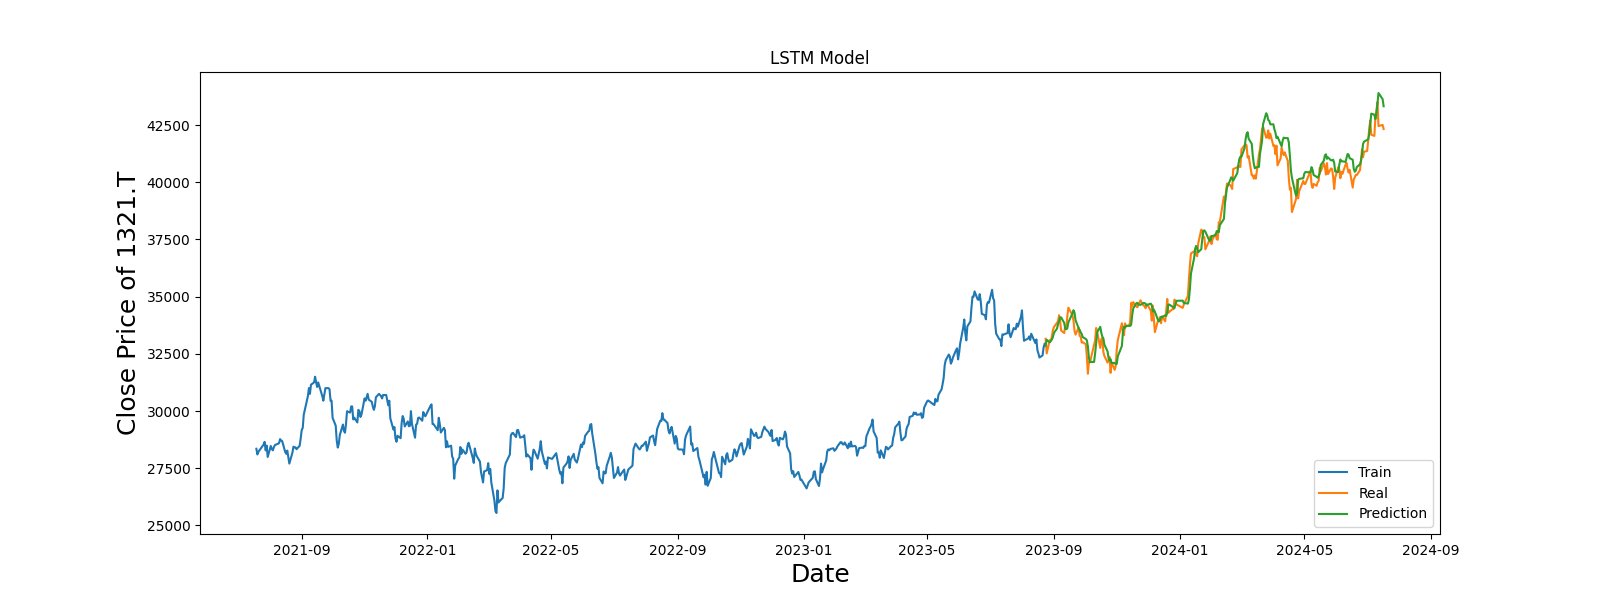
\includegraphics[width=120mm]{./exericise/image/lstm_model.png}
  \caption{exericiseのtest\_two.pyの実行結果}
  \label{twopython}
\end{figure}

\indent また、実際にこのモデルとStreamlitを用いて、次のようなページを作成した。\\
\paragraph{WebページのURL:}\url{https://finance-svkvjevmpsyc9f9ru8yefz.streamlit.app/} \\

\indent 上記のページでは、図\ref{Streamlit}のように3年間の株価データを表示し、それを用いて株価を予測するグラフを表示できる。 \\
\indent 図\ref{twopython}には、訓練データ、実際のデータ、予測データの3つの線が示されている。青色の線は訓練データを表し、オレンジ色の線は実際のデータ、緑色の線はLSTMモデルによる予測データを示しているものである。軸ラベルはそれぞれ横軸が日付(Date)、縦軸が1321.Tの終値(Close Price of 1321.T)であり、縦軸の単位は円である。

\begin{figure}[htbp]
  \centering
  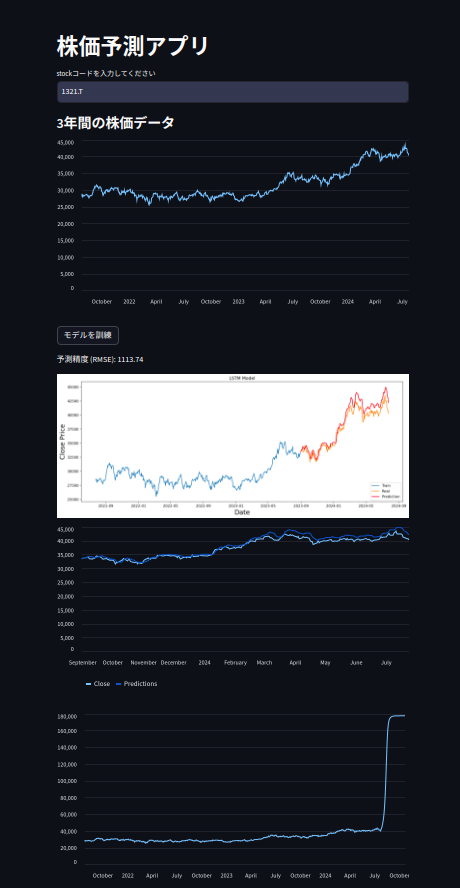
\includegraphics[width=80mm]{./image/image.png}
  \caption{Streamlitを用いたWebページ}
  \label{Streamlit}
\end{figure}
\clearpage
\section{考察}
\indent 今回の実験を通じて、LSTMモデルが1321.Tの終値予測に対して高い精度を持つことがわかった。特に2023年以降のデータにおいて、予測データと実際のデータが非常に近い値を示していることが確認できる。近い値を得ることができた理由としては、LSTMモデルの適用により、時系列データのパターンを捉えやすくなったからである。一方で、予測における誤差もいくつか見られた。特に、急激な価格変動が発生した部分では、モデルの予測精度が低下する傾向にあった。この点については、外部要因(経済ニュースや市場のイベントなど)を考慮したモデルの改良する必要がある。\\
\indent 今後の展望としては、予測精度の向上を目指し、他の時系列予測モデルとの比較検討を行うことが挙げられる。また、予測結果を活用した投資戦略の構築にも取り組みたいと考えている。また、実験を通して得られた知見を基に、次のステップとしてさらなるモデル改良と応用研究を進める予定である。

\section{意図していた実験計画との違い}
\indent 当初の実験計画では、LSTMモデルのパラメータ調整や外部要因を考慮した予測モデルの改良に十分な時間を割くことを予定していたが、LSTMモデルのトレーニング中に予期せぬエラーが発生し、その対応に多くの時間を取られた。これにより、パラメータ調整の時間が不足した。また、株価の変動には経済ニュースや市場のイベントなどの外部要因が大きく影響するため、これらをモデルに組み込むことを計画していたが、モデルの基本的なトレーニングに多くの時間を割いたため、外部要因を考慮した実験を十分に行うことができなかった。

\section{まとめ}
\indent データマイニング班として設定したテーマ「株価予測」を通じて、多くの知見を得ることができた。特に、LSTMモデルの適用により時系列データの予測精度を高める方法について深く学ぶことができた。今回の実験では、LSTMモデルのパラメータ調整やデータ前処理の重要性を再確認し、適切なモデル構築のプロセスを実践することができた。\\
\indent 実験の結果、LSTMモデルは2023年以降の株価データに対して高い予測精度を示し、株価の変動パターンを捉える能力があることがわかった。一方で、急激な価格変動に対する予測精度が低下する課題が浮き彫りになった。この課題を解決するためには、経済ニュースや市場イベントなどの外部要因を考慮したモデルの改良が必要であると考えている。\\
\indent グループワークを通じて、メンバー間のコミュニケーションや役割分担の重要性を学んだ。計画と実行のバランスを取ることの難しさを実感し、次回以降のプロジェクトにおいては、リスク管理と柔軟な対応が重要であることを認識した。


\begin{thebibliography}{99}
  \bibitem{tech} 野村證券株式会社、証券用語解説集、テクニカル分析、(参照 2024-07-25)、\url{https://x.gd/5BDJz}。
  \bibitem{nikei} 日本取引所グループ、日経225上場投資信託 (1321) 、(参照 2024-07-25)、\url{https://x.gd/iIOfc}。
  \bibitem{yfin} yfinance API、(参照 2024-07-25)、\url{https://x.gd/TJhVS}。
  \bibitem{Sequential model} Kerasライブラリ、Sequential model、(参照 2024-07-25)、\url{https://x.gd/KzEsl}。
  \bibitem{Dense layer} Kerasライブラリ、Dense layer、(参照 2024-07-25)、\url{https://x.gd/u6kQY}。
  \bibitem{LSTM layer} Kerasライブラリ、LSTM layer、(参照 2024-07-25)、\url{https://x.gd/jkxQu}。
  \bibitem{RMSD} IT用語辞典、二乗平均平方根誤差 【RMSE】、(参照 2024-07-25)、\url{https://x.gd/s5hPZ}
  \bibitem{LSTM} AI総合研究所、LSTMとは?その仕組みや使用例をわかりやすく解説!、(参照 2024-07-25)、\url{https://x.gd/6GvLI}
  \bibitem{RNN} 株式会社 日立ソリューションズ・クリエイト、自然言語処理に使われるRNN(リカレントニューラルネットワーク)とは?、(参照 2024-07-25)、\url{https://x.gd/Hejxt}
  \bibitem{RNNandLSTM} Creative Drive、"RNNとLSTM、それぞれの特性とは?違いを解説" .2023、(参照 2024-07-25)、\url{https://x.gd/YC6Fd}
  \bibitem{AI} 株式会社VOST、“AI(人工知能)用語集” . DX/AI研 . 2023。(参照 2024-07-25)、\url{https://x.gd/bFsZG}
\end{thebibliography}
\end{document}